%\SweaveUTF8




\setkeys{Gin}{width=\textwidth}

% \newcommand{\ty}{t_y}
% \newcommand{\tx}{t_x}
% \newcommand{\mHT}{\ensuremath{\mathrm{HT}}}
% \newcommand{\tysht}{\ensuremath{\widehat{t}_{\;y}^{\;\mHT}}}

\begin{Problem}[PPS Sampling and the Horvitz--Thompson
    estimator]\label{problem:pps}
    We use the data set \code{sepe.dat} from Problem Set 1 and treat the
    $N = 800$ establishments as the finite population $U$. We want to draw a
    \PPS sample without replacement of size $n = 200$, using the number of
    full-time employees as the measure of size. The data set contains:
    \begin{description}
        \item[\normalfont{\code{empl}:}] number of full-time employees, denoted
            by $x_i$. These values are known from a register before sampling;
        \item[\normalfont{\code{expend}:}] environmental expenditures, denoted
            by $y_i$. We treat these values as unknown until an establishment
            is sampled.
    \end{description}

\begin{Subtask}
    %---------------------------------------------------------------------------
    \item Compute the first-order inclusion probabilities and draw a \PPS sample
        of $n = 200$ establishments without replacement using Brewer's method.
        If there were no certainty units, the inclusion probabilities would be
        \begin{equation*}
            \pi_i = \frac{n x_i}{\tx},
            \qquad
            \tx = \sum_{i \in U} x_i.
        \end{equation*}
        Compare these naive probabilities with the probabilities returned by
        \code{pps_probabilities()} of the \code{robsurvey} package. What do you
        observe?

        \begin{Rhint}
            Attach the packages \code{survey} and \code{robsurvey} to the
            search path. Compute the inclusion probabilities and draw the
            sample as follows:

\begin{Scode}
pps_setup <- pps_probabilities(size = sepe$empl, n = 200)
pi <- as.numeric(pps_setup)

set.seed(11)
s <- pps_draw(pps_setup, method = "brewer")
\end{Scode}
        \end{Rhint}

    \begin{Solution}
        We attach the packages to the search path and load the data:


\begin{Schunk}
\begin{Sinput}
> library("survey")
> library("robsurvey")
> sepe <- read.table("http://stat.ethz.ch/Teaching/Datasets/WBL/sepe.dat",
                     header = TRUE)
\end{Sinput}
\end{Schunk}

        The valid first-order inclusion probabilities are

\begin{Schunk}
\begin{Sinput}
> pps_setup <- pps_probabilities(sepe$empl, n = 200)
> sepe$pi <- as.numeric(pps_setup)
> summary(sepe$pi)
\end{Sinput}
\begin{Soutput}
   Min. 1st Qu.  Median    Mean 3rd Qu.    Max. 
0.00000 0.07253 0.18082 0.25000 0.36296 1.00000 
\end{Soutput}
\begin{Sinput}
> sum(sepe$pi == 1)
\end{Sinput}
\begin{Soutput}
[1] 16
\end{Soutput}
\end{Schunk}

        Hence, 
        16
        establishments are certainty units with $\pi_i = 1$.
        By contrast, the naive formula gives

\begin{Schunk}
\begin{Sinput}
> pi_naive <- 200 * sepe$empl / sum(sepe$empl)
> summary(pi_naive)
\end{Sinput}
\begin{Soutput}
   Min. 1st Qu.  Median    Mean 3rd Qu.    Max. 
0.00000 0.07102 0.17706 0.25000 0.35543 1.55791 
\end{Soutput}
\begin{Sinput}
> sum(pi_naive > 1)
\end{Sinput}
\begin{Soutput}
[1] 15
\end{Soutput}
\end{Schunk}

        Some of these values exceed one and therefore cannot be inclusion
        probabilities. The function \code{pps_probabilities()} handles this
        iteratively: certainty units are assigned $\pi_i = 1$, and the
        probabilities of the remaining units are rescaled so that
        \begin{equation*}
            0 < \pi_i \leq 1
            \qquad\text{and}\qquad
            \sum_{i \in U} \pi_i = n.
        \end{equation*}
        Thus, with certainty units present, the final probabilities are not
        simply $n x_i/\tx$ for every unit. We then draw the \PPS sample:

\begin{Schunk}
\begin{Sinput}
> set.seed(11)
> s <- pps_draw(pps_setup, method = "brewer")
> length(s)
\end{Sinput}
\begin{Soutput}
[1] 200
\end{Soutput}
\end{Schunk}
    \end{Solution}

    %---------------------------------------------------------------------------
    \item Create a survey design object for the sample from part a). Then use
        \code{svyplot()} to plot environmental expenditures against the number
        of employees. The bubble sizes represent the sampling weights
        $w_i = 1/\pi_i$. Describe the main features of the plot.

        \begin{Remark}
            For the \PPS design of part a), use

\begin{Scode}
dn_sepe <- svydesign(ids = ~1, fpc = ~pi, pps = "brewer",
                     data = sepe[s, ])
\end{Scode}

            Here, \code{fpc = ~pi} supplies the first-order inclusion
            probabilities. The option \code{pps = "brewer"} tells
            \code{survey} to use Brewer's approximation for the second-order
            inclusion probabilities needed for variance estimation. This is
            distinct from Brewer's sampling algorithm used in part a).
        \end{Remark}

    \begin{Solution}
        We define the design by

\begin{Schunk}
\begin{Sinput}
> dn_sepe <- svydesign(ids = ~1, fpc = ~pi, pps = "brewer",
                       data = sepe[s, ])
\end{Sinput}
\end{Schunk}

        Omitting \code{fpc} would instead create a with-replacement
        approximation to the design.

        The scatterplot (Figure \ref{fig:pps}) is obtained with the commands:

\begin{Schunk}
\begin{Sinput}
> svyplot(expend ~ empl, dn_sepe, inches = 0.1,
          xlab = "Number of employees",
          ylab = "Environmental expenditures")
> certainty_cut <- min(sepe$empl[sepe$pi == 1])
> abline(v = certainty_cut, lty = 2)
\end{Sinput}
\end{Schunk}

        \begin{figure}[tbp]
            \centering
            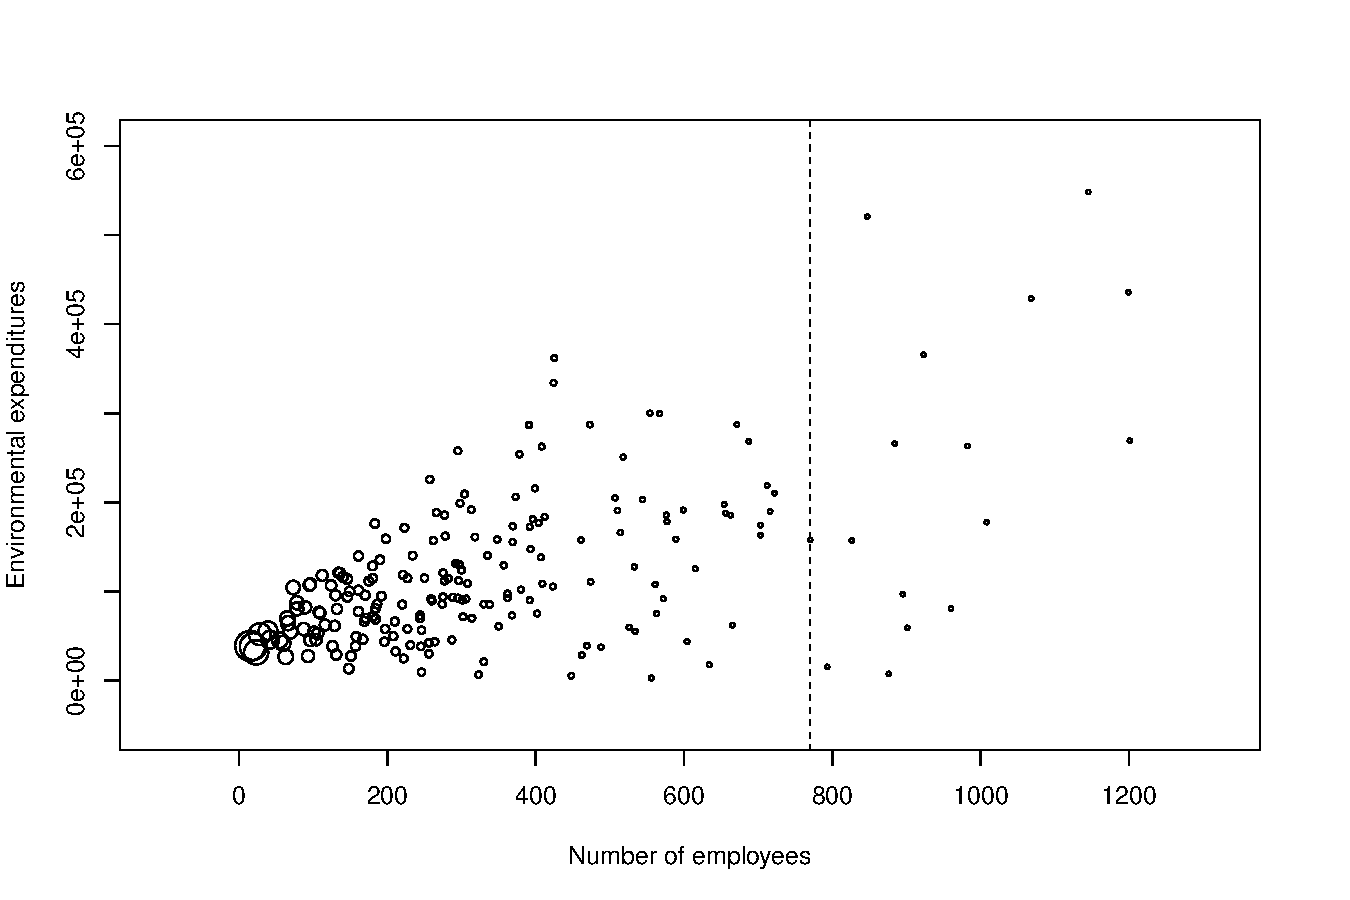
\includegraphics{problems/fig-empl_expend}
            \caption{Environmental expenditures vs. number of employees; the
            size of the bubbles is proportional to the sampling
            weights}\label{fig:pps}
        \end{figure}

        The main features are:
        \begin{itemize}
            \item Establishments with fewer employees have smaller inclusion
                probabilities and therefore larger sampling weights. They
                appear as larger bubbles.
            \item The largest establishments are certainty units. The dashed
                line marks the smallest value of \code{empl} among these units.
            \item The size measure \code{empl} is positively related to
                \code{expend}:
                0.57.
                \PPS sampling is particularly effective when $y_i$ is closely
                related to the size measure, so that the ratios $y_i/x_i$ do
                not vary too much.
        \end{itemize}
    \end{Solution}

    %---------------------------------------------------------------------------
    \item Estimate the population total of environmental expenditures,
        \begin{equation*}
            \ty = \sum_{i \in U} y_i,
        \end{equation*}
        using the Horvitz--Thompson estimator and the design from part b). Also
        compute an estimate of the standard error of the estimator.

    \begin{Solution}
        The Horvitz--Thompson estimate and its estimated standard error are
        obtained directly with

\begin{Schunk}
\begin{Sinput}
> t_y <- svytotal(~expend, dn_sepe)
> t_y
\end{Sinput}
\begin{Soutput}
          total      SE
expend 71293708 3300926
\end{Soutput}
\end{Schunk}

        The \PPS weights have an additional useful property. Because the
        inclusion probabilities were constructed from \code{empl}, the
        Horvitz--Thompson estimator reproduces its known population total:

\begin{Schunk}
\begin{Sinput}
> t_x <- svytotal(~empl, dn_sepe)
> c(estimate = coef(t_x), population = sum(sepe$empl))
\end{Sinput}
\begin{Soutput}
estimate.empl    population 
       154181        154181 
\end{Soutput}
\end{Schunk}

        The point estimate is therefore exact, but the default variance
        estimator does not automatically use this calibration information.
        We can tell \code{survey} that the supplied weights are already
        calibrated to $\tx$:

\begin{Schunk}
\begin{Sinput}
> dn_sepe_calib <- svydesign(ids = ~1, fpc = ~pi, pps = "brewer",
                             data = sepe[s, ],
                             calibrate.formula = ~ -1 + empl)
> svytotal(~empl, dn_sepe_calib)
\end{Sinput}
\begin{Soutput}
      total SE
empl 154181  0
\end{Soutput}
\end{Schunk}

        The formula has no intercept because the \PPS weights reproduce
        $\tx$, but they do not generally reproduce the population size $N$.
        The option \code{calibrate.formula} does not change the weights; it
        tells the variance estimator about an existing calibration equation.

        The estimate of $\ty$ is unchanged, while its estimated standard error
        can decrease:

\begin{Schunk}
\begin{Sinput}
> t_y_calib <- svytotal(~expend, dn_sepe_calib)
> c(estimate = unname(coef(t_y_calib)), SE_without_calibration = SE(t_y),
    SE_with_calibration = SE(t_y_calib))
\end{Sinput}
\begin{Soutput}
              estimate SE_without_calibration    SE_with_calibration 
              71293708                3300926                3313698 
\end{Soutput}
\end{Schunk}
    \end{Solution}
\end{Subtask}
\end{Problem}
